
\documentclass[a4paper, 12pt]{book}
%\documentclass[a4paper, 12pt, draft]{book}  Nalogo preverite tudi z opcijo draft, ki vam bo pokazala, katere vrstice so predolge!



\usepackage[utf8x]{inputenc}   % omogoča uporabo slovenskih črk kodiranih v formatu UTF-8
\usepackage[slovene,english]{babel}    % naloži, med drugim, slovenske delilne vzorce
\usepackage[pdftex]{graphicx}  % omogoča vlaganje slik različnih formatov
\usepackage{fancyhdr}          % poskrbi, na primer, za glave strani
\usepackage{amssymb}           % dodatni simboli
\usepackage{amsmath}           % eqref, npr.
%\usepackage{hyperxmp}
\usepackage[hyphens]{url}  % dodal Solina
\usepackage{comment}       % dodal Solina

\usepackage[pdftex, colorlinks=true,
						citecolor=black, filecolor=black, 
						linkcolor=black, urlcolor=black,
						pagebackref=false, 
						pdfproducer={LaTeX}, pdfcreator={LaTeX}, hidelinks]{hyperref}

\usepackage{color}       % dodal Solina
\usepackage{soul}       % dodal Solina

%%%%%%%%%%%%%%%%%%%%%%%%%%%%%%%%%%%%%%%%
%	DIPLOMA INFO
%%%%%%%%%%%%%%%%%%%%%%%%%%%%%%%%%%%%%%%%
\newcommand{\ttitle}{Hevristični algoritmi v RTS igri TD2020}
\newcommand{\ttitleEn}{Heuristic algoritms in RTS game TD2020}
\newcommand{\tsubject}{\ttitle}
\newcommand{\tsubjectEn}{\ttitleEn}
\newcommand{\tauthor}{Jernej Habjan}
\newcommand{\tkeywords}{hevristika, Monte-Carlo drevesno preiskovanje, CMAB}
\newcommand{\tkeywordsEn}{heuristics, Monte Carlo tree search, CMAB}


%%%%%%%%%%%%%%%%%%%%%%%%%%%%%%%%%%%%%%%%
%	HYPERREF SETUP
%%%%%%%%%%%%%%%%%%%%%%%%%%%%%%%%%%%%%%%%
\hypersetup{pdftitle={\ttitle}}
\hypersetup{pdfsubject=\ttitleEn}
\hypersetup{pdfauthor={\tauthor, jh0228@fri.uni-lj.si}}
\hypersetup{pdfkeywords=\tkeywordsEn}


 


%%%%%%%%%%%%%%%%%%%%%%%%%%%%%%%%%%%%%%%%
% postavitev strani
%%%%%%%%%%%%%%%%%%%%%%%%%%%%%%%%%%%%%%%%  

\addtolength{\marginparwidth}{-20pt} % robovi za tisk
\addtolength{\oddsidemargin}{40pt}
\addtolength{\evensidemargin}{-40pt}

\renewcommand{\baselinestretch}{1.3} % ustrezen razmik med vrsticami
\setlength{\headheight}{15pt}        % potreben prostor na vrhu
\renewcommand{\chaptermark}[1]%
{\markboth{\MakeUppercase{\thechapter.\ #1}}{}} \renewcommand{\sectionmark}[1]%
{\markright{\MakeUppercase{\thesection.\ #1}}} \renewcommand{\headrulewidth}{0.5pt} \renewcommand{\footrulewidth}{0pt}
\fancyhf{}
\fancyhead[LE,RO]{\sl \thepage} 
%\fancyhead[LO]{\sl \rightmark} \fancyhead[RE]{\sl \leftmark}
\fancyhead[RE]{\sc \tauthor}              % dodal Solina
\fancyhead[LO]{\sc Diplomska naloga}     % dodal Solina


\newcommand{\BibTeX}{{\sc Bib}\TeX}

%%%%%%%%%%%%%%%%%%%%%%%%%%%%%%%%%%%%%%%%
% naslovi
%%%%%%%%%%%%%%%%%%%%%%%%%%%%%%%%%%%%%%%%  


\newcommand{\autfont}{\Large}
\newcommand{\titfont}{\LARGE\bf}
\newcommand{\clearemptydoublepage}{\newpage{\pagestyle{empty}\cleardoublepage}}
\setcounter{tocdepth}{1}	      % globina kazala

%%%%%%%%%%%%%%%%%%%%%%%%%%%%%%%%%%%%%%%%
% konstrukti
%%%%%%%%%%%%%%%%%%%%%%%%%%%%%%%%%%%%%%%%  
\newtheorem{izrek}{Izrek}[chapter]
\newtheorem{trditev}{Trditev}[izrek]
\newenvironment{dokaz}{\emph{Dokaz.}\ }{\hspace{\fill}{$\Box$}}

%%%%%%%%%%%%%%%%%%%%%%%%%%%%%%%%%%%%%%%%%%%%%%%%%%%%%%%%%%%%%%%%%%%%%%%%%%%%%%%
%% PDF-A
%%%%%%%%%%%%%%%%%%%%%%%%%%%%%%%%%%%%%%%%%%%%%%%%%%%%%%%%%%%%%%%%%%%%%%%%%%%%%%%


%%%%%%%%%%%%%%%%%%%%%%%%%%%%%%%%%%%%%%%% 
% define medatata
%%%%%%%%%%%%%%%%%%%%%%%%%%%%%%%%%%%%%%%% 
\def\Title{\ttitle}
\def\Author{\tauthor, jh0228@fri.uni-lj.si}
\def\Subject{\ttitleEn}
\def\Keywords{\tkeywordsEn}

%%%%%%%%%%%%%%%%%%%%%%%%%%%%%%%%%%%%%%%% 
% \convertDate converts D:20080419103507+02'00' to 2008-04-19T10:35:07+02:00
%%%%%%%%%%%%%%%%%%%%%%%%%%%%%%%%%%%%%%%% 
\def\convertDate{%
    \getYear
}

{\catcode`\D=12
 \gdef\getYear D:#1#2#3#4{\edef\xYear{#1#2#3#4}\getMonth}
}
\def\getMonth#1#2{\edef\xMonth{#1#2}\getDay}
\def\getDay#1#2{\edef\xDay{#1#2}\getHour}
\def\getHour#1#2{\edef\xHour{#1#2}\getMin}
\def\getMin#1#2{\edef\xMin{#1#2}\getSec}
\def\getSec#1#2{\edef\xSec{#1#2}\getTZh}
\def\getTZh +#1#2{\edef\xTZh{#1#2}\getTZm}
\def\getTZm '#1#2'{%
    \edef\xTZm{#1#2}%
    \edef\convDate{\xYear-\xMonth-\xDay T\xHour:\xMin:\xSec+\xTZh:\xTZm}%
}

\expandafter\convertDate\pdfcreationdate 

%%%%%%%%%%%%%%%%%%%%%%%%%%%%%%%%%%%%%%%%
% get pdftex version string
%%%%%%%%%%%%%%%%%%%%%%%%%%%%%%%%%%%%%%%% 
\newcount\countA
\countA=\pdftexversion
\advance \countA by -100
\def\pdftexVersionStr{pdfTeX-1.\the\countA.\pdftexrevision}


%%%%%%%%%%%%%%%%%%%%%%%%%%%%%%%%%%%%%%%%
% XMP data
%%%%%%%%%%%%%%%%%%%%%%%%%%%%%%%%%%%%%%%%  
\usepackage{xmpincl}
\includexmp{pdfa-1b}

%%%%%%%%%%%%%%%%%%%%%%%%%%%%%%%%%%%%%%%%
% pdfInfo
%%%%%%%%%%%%%%%%%%%%%%%%%%%%%%%%%%%%%%%%  
\pdfinfo{%
    /Title    (\ttitle)
    /Author   (\tauthor, damjan@cvetan.si)
    /Subject  (\ttitleEn)
    /Keywords (\tkeywordsEn)
    /ModDate  (\pdfcreationdate)
    /Trapped  /False
}


%%%%%%%%%%%%%%%%%%%%%%%%%%%%%%%%%%%%%%%%%%%%%%%%%%%%%%%%%%%%%%%%%%%%%%%%%%%%%%%
%%%%%%%%%%%%%%%%%%%%%%%%%%%%%%%%%%%%%%%%%%%%%%%%%%%%%%%%%%%%%%%%%%%%%%%%%%%%%%%

\begin{document}
\selectlanguage{slovene}
\frontmatter
\setcounter{page}{1} %
\renewcommand{\thepage}{}       % preprecimo težave s številkami strani v kazalu
\newcommand{\sn}[1]{"`#1"'}                    % dodal Solina (slovenski narekovaji)

%%%%%%%%%%%%%%%%%%%%%%%%%%%%%%%%%%%%%%%%
%naslovnica
 \thispagestyle{empty}%
   \begin{center}
    {\large\sc Univerza v Ljubljani\\%
      Fakulteta za računalništvo in informatiko}%
    \vskip 10em%
    {\autfont \tauthor\par}%
    {\titfont \ttitle \par}%
    {\vskip 3em \textsc{DIPLOMSKO DELO\\[5mm]         % dodal Solina za ostale študijske programe
    VISOKOŠOLSKI STROKOVNI ŠTUDIJSKI PROGRAM\\ PRVE STOPNJE\\ RAČUNALNIŠTVO IN INFORMATIKA}\par}%
%    UNIVERZITETNI  ŠTUDIJSKI PROGRAM\\ PRVE STOPNJE\\ RAČUNALNIŠTVO IN INFORMATIKA}\par}%
%    INTERDISCIPLINARNI UNIVERZITETNI\\ ŠTUDIJSKI PROGRAM PRVE STOPNJE\\ RAČUNALNIŠTVO IN MATEMATIKA}\par}%
%    INTERDISCIPLINARNI UNIVERZITETNI\\ ŠTUDIJSKI PROGRAM PRVE STOPNJE\\ UPRAVNA INFORMATIKA}\par}%
%    INTERDISCIPLINARNI UNIVERZITETNI\\ ŠTUDIJSKI PROGRAM PRVE STOPNJE\\ MULTIMEDIJA}\par}%
    \vfill\null%
    {\large \textsc{Mentor}: doc.\ dr.  Matej Guid\par}%
    {\vskip 2em \large Ljubljana, 2018 \par}%
\end{center}
% prazna stran
%\clearemptydoublepage      % dodal Solina (izjava o licencah itd. se izpiše na hrbtni strani naslovnice)

%%%%%%%%%%%%%%%%%%%%%%%%%%%%%%%%%%%%%%%%
%copyright stran
\thispagestyle{empty}
\vspace*{8cm}

\noindent
{\sc Copyright}. 
Rezultati diplomske naloge so intelektualna lastnina avtorja in Fakultete za računalništvo in informatiko Univerze v Ljubljani.
Za objavo in koriščenje rezultatov diplomske naloge je potrebno pisno privoljenje avtorja, Fakultete za računalništvo in informatiko ter mentorja.

\begin{center}
\mbox{}\vfill
\emph{Besedilo je oblikovano z urejevalnikom besedil \LaTeX.}
\end{center}
% prazna stran
\clearemptydoublepage

%%%%%%%%%%%%%%%%%%%%%%%%%%%%%%%%%%%%%%%%
% stran 3 med uvodnimi listi
\thispagestyle{empty}
\vspace*{4cm}

\noindent
Fakulteta za računalništvo in informatiko izdaja naslednjo nalogo:
\medskip
\begin{tabbing}
\hspace{32mm}\= \hspace{6cm} \= \kill




Tematika naloge:
\end{tabbing}
Besedilo teme diplomskega dela študent prepiše iz študijskega informacijskega sistema, kamor ga je vnesel mentor. V nekaj stavkih bo opisal, kaj pričakuje od kandidatovega diplomskega dela. Kaj so cilji, kakšne metode uporabiti, morda bo zapisal tudi ključno literaturo.
\vspace{15mm}






\vspace{2cm}

% prazna stran
\clearemptydoublepage

% zahvala
\thispagestyle{empty}\mbox{}\vfill\null\it%
\noindent
Zahvaljujem se celi družini pri podpori pri študiju, sostanovalcem v Ljubljani in vsem kolegom, ki so mi priskočili na pomoč.
Prav tako se zahvaljujem mentorju doc.\ dr.  Mateju Guidu za vodenje.

\rm\normalfont

% prazna stran
\clearemptydoublepage


%%%%%%%%%%%%%%%%%%%%%%%%%%%%%%%%%%%%%%%%
% kazalo
\pagestyle{empty}
\def\thepage{}% preprecimo tezave s stevilkami strani v kazalu
\tableofcontents{}


% prazna stran
\clearemptydoublepage

%%%%%%%%%%%%%%%%%%%%%%%%%%%%%%%%%%%%%%%%
% seznam kratic

\chapter*{Seznam uporabljenih kratic}  % spremenil Solina, da predolge vrstice ne gredo preko desnega roba

\begin{comment}
\begin{tabular}{l|l|l}
  {\bf kratica} & {\bf angleško} & {\bf slovensko} \\ \hline
  % after \\: \hline or \cline{col1-col2} \cline{col3-col4} ...
  {\bf CA} & classification accuracy & klasifikacijska točnost \\
  {\bf DBMS} & database management system & sistem za upravljanje podatkovnih baz \\
  {\bf SVM} & support vector machine & metoda podpornih vektorjev \\
  \dots & \dots & \dots \\
\end{tabular}
\end{comment}

\noindent\begin{tabular}{p{0.1\textwidth}|p{.4\textwidth}|p{.4\textwidth}}    % po potrebi razširi prvo kolono tabele na račun drugih dveh!
  {\bf kratica} & {\bf angleško}                             & {\bf slovensko} \\ \hline
  {\bf MCTS}      & Monte Carlo tree search               & Monte-Carlo drevesno preiskovanje \\
  {\bf UCB} & upper confidence bound & zgornja meja zaupanja \\
  {\bf RAVE} & rapid action value estimation & hitra ocena učinka \\
  {\bf CMAB} & combinatorial multi-armed bandit & kombinatorni več-rokovni bandit \\
   {\bf UE4} & game engine Unreal Engine 4 & celostni pogon Unreal Engine 4 \\
     {\bf RTS} & real-time strategy & realno-časovna strateška \\
  
  
\end{tabular}


% prazna stran
\clearemptydoublepage

%%%%%%%%%%%%%%%%%%%%%%%%%%%%%%%%%%%%%%%%
% povzetek
\addcontentsline{toc}{chapter}{Povzetek}
\chapter*{Povzetek}

\noindent\textbf{Naslov:} \ttitle
\bigskip

\noindent\textbf{Avtor:} \tauthor
\bigskip

%\noindent\textbf{Povzetek:} 
\noindent V okolju UE4 smo razvili algoritem, ki namesto klasičnega programiranja umetne inteligence v RTS igrah uporablja hevrističen algoritem,ki sam ugotovi, katera je optimalna odločitev v določeni situaciji in jo za tem izvede, pri katerem je problem velik preiskovalni prostor, ki se pojavlja v RTS igrah.
Pri igri Trump Defense 2020, narejeni v UE4 smo uporabili algoritem Monte-Carlo drevesno preiskovanje, ki deluje na principu hevrističnega preiskovanja prostora, kjer imamo prostor stanj (graf, drevo), množico dosegljivih stanj in povezave med stanji.
Najbolj uspešno se je izkazal CMAB izpeljanka algoritma MCTS, ki je dajal poudarek na računanju vrednosti akcije proti številu simulacij.

\bigskip

\noindent\textbf{Ključne besede:} \tkeywords.
% prazna stran
\clearemptydoublepage

%%%%%%%%%%%%%%%%%%%%%%%%%%%%%%%%%%%%%%%%
% abstract
\selectlanguage{english}
\addcontentsline{toc}{chapter}{Abstract}
\chapter*{Abstract}

\noindent\textbf{Title:} \ttitleEn
\bigskip

\noindent\textbf{Author:} \tauthor
\bigskip

%\noindent\textbf{Abstract:} 
\noindent In the UE4 environment, we developed an algorithm that uses a heuristics instead of classically programmed artificial intelligence, which itself determine the optimal decision in a given situation and performs it, with the problem being a large investigative space that appears in RTS games.
In the Trump Defense 2020 game, made in UE4, we used the Monte Carlo tree search algorithm to investigate trees, which operates on the principle of heuristic space exploration, where we have a space of states (graph, tree), a multitude of accessible states and connections between states.
The most successful was the CMAB implementation of the MCTS algorithm, which emphasized calculating the value of the action against the number of simulations.


\bigskip

\noindent\textbf{Keywords:} \tkeywordsEn.
\selectlanguage{slovene}
% prazna stran
\clearemptydoublepage

%%%%%%%%%%%%%%%%%%%%%%%%%%%%%%%%%%%%%%%%
\mainmatter
\setcounter{page}{1}
\pagestyle{fancy}

\chapter{Uvod}
Računalnik, ki igra proti človeškem nasprotniku lahko sprogramiramo na klasičen način pogoj - akcija. Tako so narejene klasične realno-časovno strateške igre, vendar gre veliko časa za implementacijo posameznih sovražnikovih napadov in nabiranju virov.
Lahko pa razvijemo algoritem, ki sam ugotovi, katera je optimalna odločitev v določeni situaciji in jo za tem izvede.
Na preprostih problemih z malo odločitvami in kratkimi igrami kot je igra križci in krožci, lahko izberemo preprostejše algoritme kot je algoritem Minimax, kjer igralec hoče povečati svojo možnost zmage, nasprotnik pa mu hoče to možnost zmanjšati.
Obstajajo tudi algoritmi, ki se naučijo igre iz učne množice, ki predstavlja nekaj iger, pri tem pa računalnik ugotovi zakonitosti igre in način igranja.
Taki algoritmi so nevronske mreže ali globoke nevronske mreže, ki pa so zelo računsko potratni, vendar vračajo izjemne rezultate. 
Lahko pa uporabimo algoritem Monte-Carlo drevesno preiskovanje, ki deluje na principu hevrističnega preiskovanja prostora, kjer imamo prostor stanj (graf, drevo), množico dosegljivih stanj in povezave med stanji.
Algoritem bom uporabil na svoji igri narejeni v celostnem pogonu Unreal Engine 4 imenovani Trump Defense 2020.


Razvijanje inteligentnega agenta v realno-časovnih igrah je problem, s katerim se mora soočiti večina razvijalcev teh iger, agentove akcije so pa pogosto predvidljive, saj se človeški igralec nauči njihovih načinov delovanja in jih tako lažje premaga.
Če pustimo agentu, da sam opravlja akcije nekontrolirano, bo izvajal naključne akcije, ki so pa slabše kot vnaprej definirana taktika.
Če pa agentu podamo hevristiko, po kateri se mora ravnati, bo poskušal izvesti čim boljše akcije, vendar bo to trajalo zelo dolgo, saj bo moral preiskati cel preiskovalni prostor, ki pa pri realno-časovnih strateških igrah zna biti zelo velik.
Da bi agent lahko poiskal cel prostor, bi ga morali zelo abstraktirati, vendar še takrat se moramo posluževati algoritmov kot je Monte-Carlo drevesno preiskovanje, ki uporablja naključnost, s katero se pomika skozi preiskovalni prostor.
S takim algoritmom lahko dosežemo inteligentnega agenta, ki se prilagaja nasprotnikovim akcijam, vsako igro izbira nov način igranja in deluje dovolj hitro brez daljšega učenja na superračunalnikih, kot to potrebujejo nevronske mreže.

%%%%%%%%%%%%%%%%%%%%%%%%%%%%%%%%%%%%%%

\chapter{Realno-časovne strateške igre}
Njihov cilj je gradnja ekonomije, vojske in z njo premagati nasprotnika z porušenjem njihovih hiš.
Razlike realno-časovnih strateških iger od šaha so naslednje:
Akcije se izvršujejo hkrati in niso potezne
Poteze lahko trajajo dlje časa(hoja do hiše)
Igra je “realno-časovna” kar pomeni, da se mora v vsakem trenutku igralec odločiti za potezo, za katero lahko pri šahu razmišlja dlje časa (vsakih 42 milisekund)
Večina iger je le delno vidnih, kjer vidimo nasprotnikove objekte samo ob določenih pogojih
Prostor preiskovanja akcij je veliko večja.


\section{Izdelava strateške igre}
Igro moram izdelati v celostnem pogonu Unreal Engine 4.
Igra bo realno-časovna, kar pomeni, da jo moram dobro optimizirati, če hočem poganjati hevristične preiskovalne algoritme. V tem okolju bom lažje zasnoval grafično prezentacijo algoritma.
\subsection{Celostni pogon Unreal Engine 4}
Unreal Engine 4 je odprtokodni program podjetja Epic Games, ki je namenjen hitri izdelavi računalniških iger. Obstajajo še drugi celostni pogoni kot je Unity.\\
Razliko med tema pogonoma je dobro predstavil Marko Kladnik \cite{diploma2}.\\
Unreal Engine 4 omogoča hitro ustvarjanje iger s pomočjo posebnih diagramov (angl. blueprint) in hkrati podpira programski jezik C++, ki ga uporabimo za hitro izvedbo velikega števila matematičnih izrazov.\\
Pogon podpira odločitvena drevesa, v katera lahko sprogramiramo računalnikovo delovanje ob določenih pogojih, vendar je v igri Trump Defense 2020 narejena inteligenca računalnika s hevrističnim algoritmom Monte-Carlo drevesno preiskovanje.\\
Izdelati moram poganjalca algoritma, ki bo izbral določen algoritem in z njim igral proti nasprotniku ali proti človeškem igralcu.\\
Prav tako moram izdelati osebke in njihove akcije (npr. postavi hišo).
Te osebke bom pa hranil v stanju igre, ki pa ga algoritem uporablja, ki je abstrakcija za to, kateri osebki in akcije so trenutno na voljo.

\section{Trump Defense 2020}
Opis igre in problema:
Realno-časovna igra, kjer imamo na voljo 2 rase - Humans in Aliens.
Svet je razdeljen na 2 mreži, kjer je mreža za gradnjo in postavljanje stavb velika 32 x 32 kvadratkov, mreža za hojo pa 8 x 8 kvadratkov. Tipične velikosti mape so od 64 x 64 do 256 x 256 kvadratkov. Kontroliramo lahko do 200 enot na igralca, kjer imamo za vsako raso približno 30 - 35 različnih enot in stavb. Tu je razvidna kompleksnost igre, ki je s preprostim preiskovanjem prostora ne premagamo.\\
Predpostavke:
\begin{itemize}
\item Da je okrog enote največ 16 sovražnih enot,
\item enota se lahko premakne na sosednih 8 kvadratkov, čeprav se enota v realnosti lahko  premakne kamorkoli na mapi.
\item Delavec lahko postavi hišo samo na trenutno lokacijo (njegova lokacija)
\end{itemize}
\subsection{Izzivi realno-časovnih iger}
Zgodnje raziskave realno-časovnih iger so ugotovile naslednje izzive:
\begin{itemize}
\item Upravljanje z viri
\item Izbira akcij ob nevednosti
\item Prostorsko in časovno razmišljanje
\item Sodelovanje med večimi agenti
\item Modeliranje nasprotnika in učenje
\item Nesporno načrtovanje v realnem času
\end{itemize}

Zdajšni izzivi:
\begin{itemize}
\item Planiranje:
Planiranje v realno-časovni igri je vidno kot več nivojev abstrahiranega stanja igre. Višji kot je nivo, bolj dolgoročni so cilji, kot naprimer gradnja ekonomije, na nižjem nivoju je pa premik posamezne enote ipd.
\item Učenje:
Predhodno učenje, ki uporablja posnetke že odigranih iger,
Učenje v igri, ki uporablja po večini spodbujevalno učenje in modeliranje nasprotnika.
Učenje med igrami
\item Negotovost:
Negotovost nastane zaradi nevidnosti nasprotnika in njegovih potez v vsakem trenutku. Prav tako pa ne vemo akcij, ki jih bo nasprotnik naredil, zato zgradimo drevo, ki nam pove kaj je najverjetneje da bo nasprotnik naredil.
\item Prostorsko in časovno razumevanje:
Prostorsko razumevanje je usmerjeno k postavljanju stavb in pozicijo vojske za obrambo in napad.
Časovno razumevanje je pa usmerjeno k ugotavljanju, kdaj je primerna izdelava hiš za ekonomijo in kdaj pa za napad.
\item Izkoriščanje znanja domen:
Izkoriščanje znanje botov. StarCraft je kompleksen, in to ostaja še odprt problem
\item Razdelitev nalog~\ref{pic1}:
Strategija, ki je najvišja abstrakcija (3 min planiranje)
Taktika, ki je implementacija trenutne strategije (pozicija vojske, hiš - 30 sec planiranje)
Reakcijska kontrola, ki je implementacija taktike, ki je osredotočena na posamezno enoto
Analiza terena, ki se osredotoča na strnjena območja in na višinsko prednost
Pridobivanje znanja, s katerim pridobivamo informacije o taktiki nasprotnika.

\begin{figure}[h]
	\begin{center}
		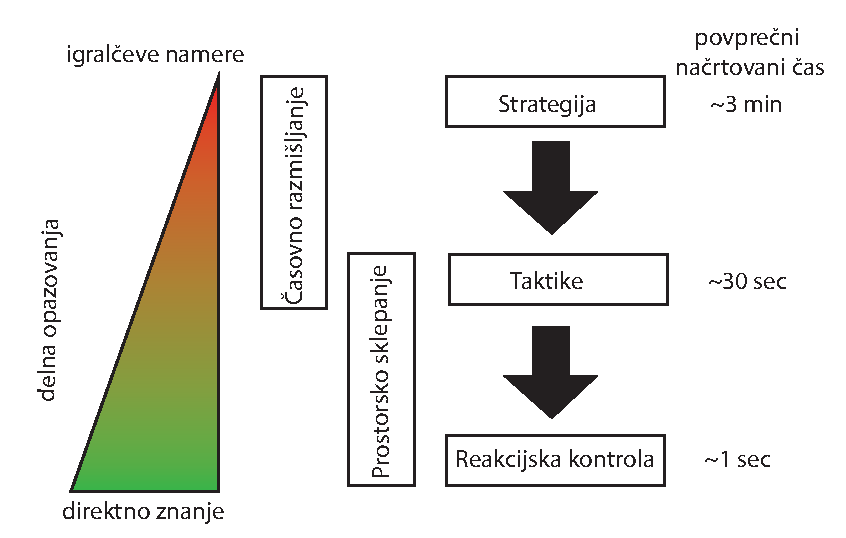
\includegraphics[width=0.6\textwidth]{RazdelitevNalog.pdf}
	\end{center}
	\caption{Razdelitev nalog.}
	\label{pic1}
\end{figure}

Pogosto razdelimo odločanje na dva dela:
\begin{itemize}
\item Micro, kjer kontroliramo enote posamezno
\item Macro, kjer se osredotočimo na ekonomijo in izdelavo enot
\end{itemize}
\end{itemize}
\section{Obstoječa dela na področju umetne inteligence v realno-časovnih igrah}
Izzivi realno-časovnih iger in obstoječa dela so povzetek članka iz leta 2013 A Survey of Real-Time Strategy Game AI Research and Competition in StarCraft~\cite{survey_real_time_strategy_ai_research_starcraft}

\subsection{Strategija}
To je še odprt problem, ki je v strateških igrah velikokrat uporabljen princip “hard-coded” ali direktnega kodiranja strategije, ki uporabljajo avtomate končnih stanj, kjer lahko razbijemo delovanje na več stanj kot so napadanje, nabiranje surovin, popravilo itd. in hitro menjavanje med njimi. Direktno kodiranje je prinesel dobre uspeške, vendar se lahko igralec nauči strategije in ga tako agenta hitro porazi.
Planirani pristopi ponujajo večjo prilagodljivost kot direktno kodirani.
Prav tako so izvajali nadzorovano učenje na podlagi podatkovnega rudarjenja na označenih StarCraft posnetkih, s katerih so se naučili sekvenco postavitve stavb.
Prav tako je pa tu problem, da je StarCraft le delno viden, kjer le del algoritmov deluje ob nevednosti nasprotnikovih akcij.
\subsection{Taktika}
Razdeljena je na naslednje sklope:
\begin{itemize}
\item Analiza terena, kjer je Perkins apliciral Voronoi dekompozicijo na mapo, ki jo razbije na manjše delčke glede na pozicijo ožin.
	Hale je predstavil mapo z 2D geometrijsko navigacijsko mrežo
\item Odločanje, kjer so bili uporabljeni različni pristopi kot strojno učenje in iskalna drevesa, skriti markovski modeli itd.
	Nekateri so uporabili spodbujevalno učenje in nevronske mreže, ki zagotovi ponovljivost taktike.
	Pri uporabi preiskovalnega drevesa je potrebno zagotoviti dovolj veliko abstrakcijo igre.
\end{itemize}

\subsection{Reakcijski nadzor}
Se osredotoča na nadzor enot, da jim povečamo izkoristek v kompleksnih bitkah na večnivojskem terenu.
Raziskovalci so izdelali vplivne karte, uporabili A* za izogib pastem, uporaba navigacije za izogibanje nasprotnikovega ognja itd.
Pri tehnikah, ki temeljijo na raziskavi terena je problem veliko število parametrov, ki so ga nekateri razreševali z uporabo spodbujevalnega učenja, vendar lahko model hitro konvergira k lokalnem maksimumu.
Pri raziskovalnih drevesih je Chirchill predstavil varacijo alpha-beta iskanja, ki deluje za hkratne gibe in za akcije, ki trajajo dlje časa.
\subsection{Celostni pristopi}
Področje ni dovolj raziskano, vendar pristopi, ki problem razbijejo na manjše dele v praksi vračajo boljše rezultate.
Celostni pristopi, izvedeni z Monte-Carlo drevesnim preiskovanjem so bili izvedeni na manjših realno-časovnih strateških igrah.

\section{Odprta vprašanja o umetni inteligenci v realno-časovnih igrah}
Zaenkrat nimamo agenta, ki bi ugotavljal svoje taktike, kot naprimer spuščanje enot v sovražnikovo bazo na podlagi nasprotnikove strategije.
\begin{itemize}
\item Učenje in prilagajanje
Prilagajanje na nasprotnikovo strategijo, učenje te strategije.
Trenutni agenti se odločajo o strategiji glede na direktno kodiranih pogojih.
Učenje na podlagi izkušenj.
Učenje iz posnetkov.
\item Planiranje
Nadzorno načrtovanje pod omejitvami v realnem času. Razvite so metode za manjše strateške igre.
Nadzorno načrtovanje pod nevednostjo zaradi delno vidne mape
\item Integracija
Integracija modulov za obravnavanje posameznih delov igre
\item Znanje o domeni
Znamo uporabiti določena znanja kot so zaporedje postavljanja stavb, ampak ne znamo še zakodirati strategije za ostale tipe iger.
\end{itemize}

%%%%%%%%%%%%%%%%%%%%%%%%%%%%%%%%%%%%%%

\chapter{Algoritmi}
Ko bom imel izdelano ogrodje strateške igre, se bom lahko posvetil algoritmom.
Preiskal bom naslednje algoritme:
\section{Monte-Carlo drevesno preiskovanje}
Implementacija algoritma v UE4 v Python programskem jeziku preko vtičnika Unreal Engine Python, ki bo poenostavila berljivost algoritma in lažjo implementacijo odprtokodnih rešitev različnih variacij MCTS algoritma, kot tudi nevronske mreže za uteženo izbiranje akcij.
\subsection{UCB1, CAB, Naive MCTS}
Izmed MCTS algoritmov bom prvo implementiral UCB1 algoritem.
\begin{equation}
R(s,a) = Q(s,a) + c\sqrt{\dfrac{\ln{s}}{N(s,a)}}
\label{eq:1}
\end{equation}
UCB1 se od ostalih algoritmov razlikuje z ocenjevalno funkcijo, ki je pa pri UCB1 najlažja.
Prav tako bom implementiral izpeljanke algoritmov CAB in Naiven MCTS, ki mi bosta pomagala primerjati algoritme med sabo in izbiro najboljše rešitve.

\subsection{Nevronske mreže}
Prav tako se bo za uteženo izbiro akcij v vozliščih implementirala variacija nevronske mreže.


Prav tako bom moral hkrati opisati, zakaj sem se za kateri algoritem odločil.
%%%%%%%%%%%%%%%%%%%%%%%%%%%%%%%%%%%%%%

\chapter{Implementacija algoritmov}
Ko bom imel algoritem dokončan, ga bom lahko implementiral v igro.
\section{implementacija naključnosten algoritma}
Sprva bom implementiral naključnosten algoritem, ki bo naključno izbiral akcije dveh igralcev. To mi bo dovolilo da preverim, ali se vse akcije uspešno izvajajo in da se stanje igre uspešno prenaša iz cikla v cikel. Prav tako mi bo omogočilo pripravo Python okolja, v katerega bom moral pridobiti vse podatke o igri, ki so potrebni za obdelavo.
\section{implementacija MCTS}
Nadgradnja naključnostnega algoritma bo osnoven MCTS, ki bo uporabljal UCB1 ocenjevalno funkcijo za izbiro vozlišča.
\section{sprememba preiskovalnega parametra pri ocenjevanju}
Tu bom še spremenil razne ocenjevalne funkcije algoritmov, spremenil preiskovalni parameter, ki določa utež preiskovanja prostora proti direktnemu odločanju.
Prav tako bom tu implementiral še nevronske mreže, ki bodo določale utež za izbiro vozlišča.

%%%%%%%%%%%%%%%%%%%%%%%%%%%%%%%%%%%%%%
\chapter{Ovrednotenje rezultatov}

\section{Simulacija igre računalnika proti računalniku}
Rezultate bom ovrednotil tako, da bom različne algoritme poganjal drug proti drugemu in si hkrati beležil število zmag.
Ko bo število iger dovolj veliko, da bo rezultat stabilen bom postopek ponovil proti drugemu algoritmu.
\begin{center}
	\begin{tabular}{ | l | l | l | l | p{5cm} |}
		\hline
		& UCB1 & CAB & Naive MCTS &Opis \\ \hline
		UCB1 & 22\% & 22\% & 22\% & Opis1. \\ \hline
		CAB & 22\%  & 22\%  & 22\%  &Opis2. \\ \hline
		Naive MCTS & 22\%  &22\%  & 22\%  & Opis3. \\ \hline
		
	\end{tabular}
\end{center}
\section{Igranje računalnika proti človeku}
Nakoncu bom poskusil algoritem testirati proti znancem, ki bodo pa podali subjektivno oceno o težavnosti algoritma in število zmag algoritma proti njim.
Tako bom izvedel, ali je algoritem koristen proti človeškim igralcem in ali se lahko človeški igralec nauči taktike, ki deluje najbolje proti algoritmu, če ta vedno izbira podobne akcije.


Pri simulaciji računalnika proti računalniku, se bom osredotočil na rezultate kot so naprimer povprečno število simulacij pri MCTS algoritmu in konsistentnost ukazov.
Pri igranju proti človeku bom pa analiziral nekaj odločitvenih dreves ki jih je računalnik zgeneriral in ocenil odločitve na podlagi mojega predznanja igre.

\begin{center}
	\begin{tabular}{ | l | l | l | l | p{5cm} |}
		\hline
		& UCB1 & CAB & Naive MCTS &Opis \\ \hline
		Oseba1 &22\% &22\%  & 22\%  & Opis1. \\ \hline
		Oseba2 & 22\% & 22\%  & 22\%  &Opis2. \\ \hline \hline
		Rezultati & 22\%  & 22\%  &22\%  & \\
		\hline
	\end{tabular}
\end{center}

\chapter{Zaključek}
V zaključku bom povzel rezultate računalnika proti računalniku, kot tudi uspešnost algoritmov proti človeškim igralcem.
Povzel bom koristnost hevrističnih algoritmov na realno-časovnih strateških igrah in vpliv abstrakcije prostora.


\newpage %dodaj po potrebi, da bo številka strani za Literaturo v Kazalu pravilna!
\ \\
\clearpage
\addcontentsline{toc}{chapter}{Literatura}
\bibliographystyle{plain}
\bibliography{literatura}


\end{document}

